\documentclass[12pt]{article}
\usepackage[utf8]{inputenc}


\usepackage{amsthm}
\usepackage{amsmath}
\usepackage{amssymb}
\usepackage[colorlinks,citecolor=blue,urlcolor=blue,filecolor=blue,backref=page]{hyperref}
\usepackage{graphicx}
\usepackage[authoryear, longnamesfirst, sort&compress]{natbib}
%\shortcites{flaxman2020b, thompson2019, Nouvellet2018, verity2020, cintron-Arias2009, ferguson2006, gostic2020}



\begin{document}


\centerline{\bf \large{Bringing proxies to the calendar scale:}}

\bigskip
\begin{enumerate}
\item Assume that we have an age depth model.  That is, given the parameters $\theta, x$, we have an age-depth model
$G( d, \theta, x)$ for any given depth $d$.  In Bacon or Plum, $\theta$ is the surface date and $x$ are the accumulation rates of the piece-wise linear age-depth model $G$. In a Bayesian inference setting, $\theta, x$ are unknown and modeled as random variables, $\Theta, X$.  The posterior distribution of $\Theta, X$ is obtained and therefore a probabilistic age-depth model is in fact obtained
$$
G( d, \Theta, X) .
$$
A MCMC posterior sample is obtained (the .out file without the memory and energy) for $\Theta, X$, be it $(\theta^{(1)}, x^{(1)}), (\theta^{(2)}, x^{(2)}), \ldots , (\theta^{(T)}, x^{(T)})$.  An MC ensamble of age-depths models, $G( d, \theta^{(t)}, x^{(t)})$, are obtained from which the posterior distribution of $G( d, \Theta, X)$ is obtained for a grid of depths $d$ (i.e. the Bacon plots).

\item Assume that we have $k$ proxy data in the core, that is, measurements $p_k(d)$ of proxy $k$ at each depth $d$.

\item To bring the proxies to the age scale one needs
$$
q_k(g) = p_k( G^{-1} ( g, \Theta, X ) ),
$$
where $G^{-1} ( g, \Theta, X )$ is the inverse of $G$ and $g$ is any calendar age.  $q_k(g)$ is a well defined r.v.

\item Note that a MC posterior sample for   $q_k(g)$ is easily obtained with
$$
q_k^{(t)}(g) = p_k( G^{-1} ( g, \theta^{(t}, x^{(t)} ) ).
$$
That is:
\begin{enumerate}
\item For each iteration in the MCMC sample for $\Theta, X$, calculate $G( d, \theta^{(t)}, x^{(t)})$.
\item For a grid of calendar ages $g_i$s, calculate the inverses $G^{-1} ( g, \theta^{(t)}, x^{(t)} )$, that is,
depth $d_i$ such that $G( d_i, \theta^{(t)}, x^{(t)}) = g_i$.
\item Then $q_k^{(t)}(g_i) = p_k(d_i)$
\end{enumerate}

\item $q_k^{(t)}(g_i)$ is a (posterior) MC ensable of proxies, from which the posterior distribution of $q_k(g_i)$ may be otained (the histogram of $q_k^{(t)}(g_i)$ !) and also an evolution of the proxy may be plotted, now in the age scale.

\end{enumerate} 

\begin{figure}
\begin{tabular}{c c}
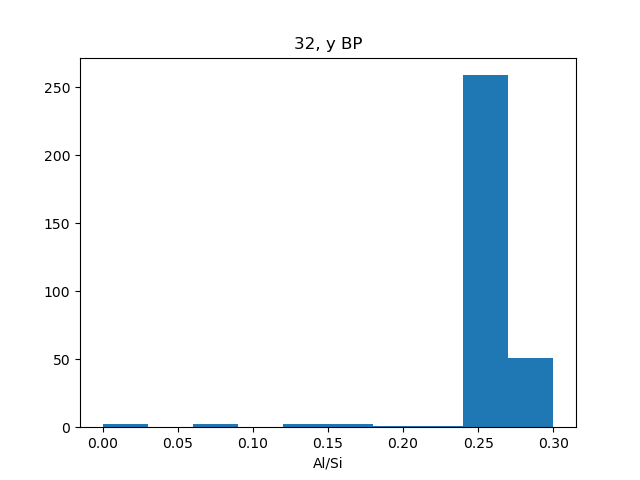
\includegraphics[scale=0.5]{LL14_AlSi_32} &
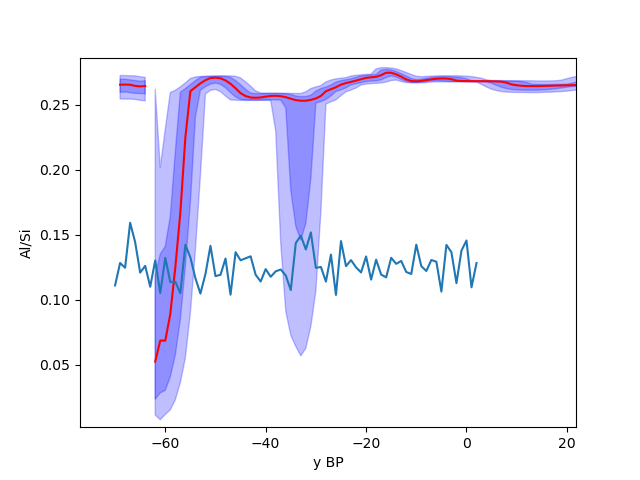
\includegraphics[scale=0.5]{LL14_AlSi} \\
\end{tabular}
\caption{LL14 Nothern CA lake (Lyssana): Histogram for the posterior distribution of proxy Al/Si at age 32 (left) and ensamble of posterior distributions for the same proxy at many ages (right), using quantiles 0.1, 0.25, 0.5 (median, read line), 0.75 and 0.9.  The additional time series plotted is the `intensity' in atmospheric rivers, plotted with arbitrary scale.}

\end{figure}



\end{document}

